% =============================================================
% SECTION IV: METHODOLOGY
% =============================================================
\section{Methodology}
\label{sec:methodology}

This section outlines the high-level approach behind NyayaSahaya's core subsystems. Implementation specifics, parameters, and sensitive operational details are intentionally abstracted.

\subsection{Dual-Path Retrieval and Contextual Grounding}

NyayaSahaya uses a dual-path strategy to support both general legal questions and document-specific inquiries. A routing component selects an appropriate pathway based on the presence of document context. One path retrieves relevant legal context from a curated knowledge base, while the other focuses on the user-provided document to preserve its full contextual structure. The two paths converge into a unified response pipeline that produces grounded, user-facing guidance. Fig.~\ref{fig:rag_pipeline} provides a conceptual view of this dual-path flow.

\begin{figure*}[!t]
\centering
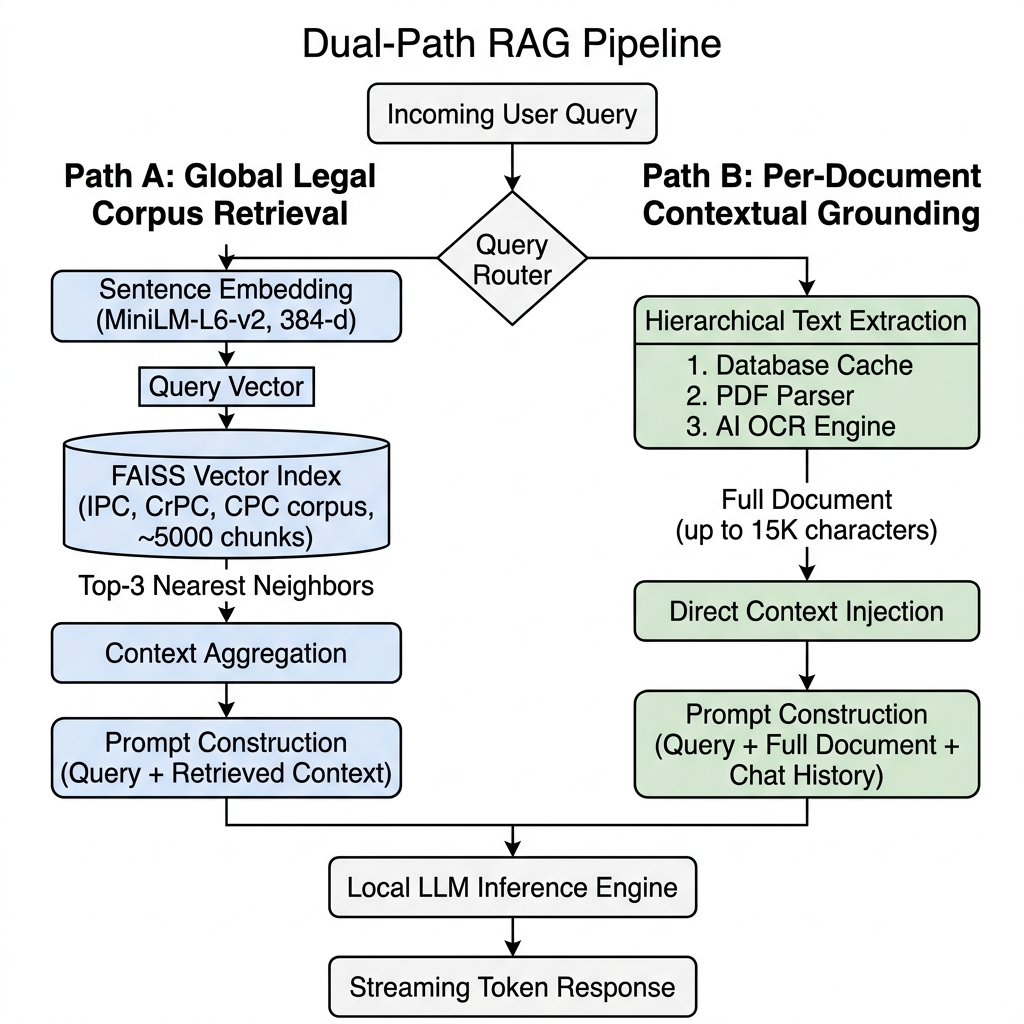
\includegraphics[width=0.70\textwidth]{figures/rag_pipeline.png}
\caption{Abstract dual-path retrieval and grounding flow. One path emphasizes global context retrieval while the other emphasizes document-specific grounding, converging into a single response pipeline.}
\label{fig:rag_pipeline}
\end{figure*}

\subsection{Authentication and Integrity}

The platform employs a trusted edge component to verify user presence and to emit signed integrity assertions. These assertions are validated by the orchestration layer and linked to document actions, enabling auditable workflows without exposing sensitive verification steps to the client interface. The resulting trust chain allows document actions to be traced to verified interactions without revealing the underlying verification mechanism.

\subsection{Document Analysis}

Document analysis produces structured summaries, key term highlights, and risk-oriented observations. The pipeline balances automated extraction with consistency checks and re-analysis triggers to avoid stale or incomplete outputs while keeping operational details confidential. Outputs are designed for practical review, emphasizing clarity and traceable rationale rather than technical internals.
